\documentclass{article}

\usepackage{pgfplots}

\begin{document}

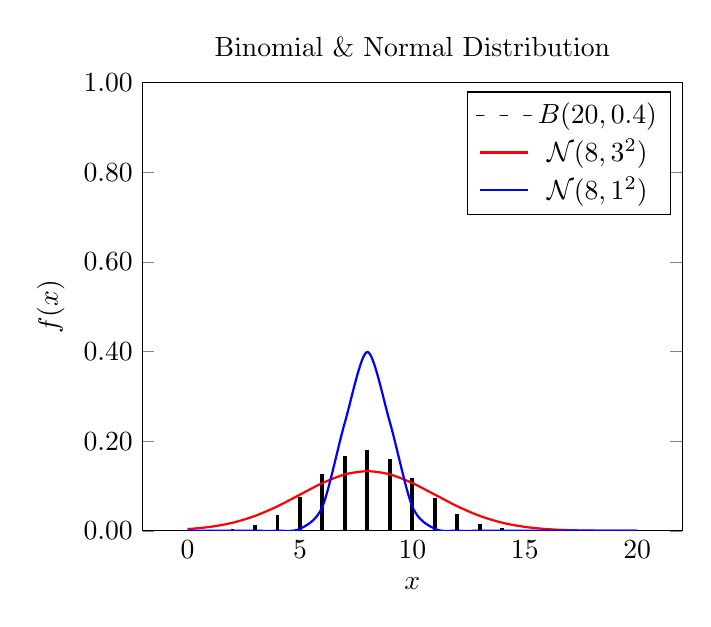
\begin{tikzpicture}
\begin{axis}
[
    % Define probability distribution functions
    declare function={
        binom(\n,\p) = \n!/(x!*(\n-x)!)*\p^x*(1-\p)^(\n-x);
        normal(\m,\s) = 1/(\s*sqrt(2*pi))*exp(-((x-\m)^2)/(2*\s^2));
    },
    % Plotting options
    title=Binomial \& Normal Distribution,
    xlabel={$x$},
    ylabel={$f(x)$},
    ymin=0,
    ymax=1,
    samples at={0,...,20},
    xtick style={draw=none},
    yticklabel style={
        /pgf/number format/fixed,
        /pgf/number format/fixed zerofill,
        /pgf/number format/precision=2,
    },   
]
  
% Plot Binomial Distribution
\addplot [ybar=0pt,bar width=1pt,fill=black] {binom(20,0.4)};  
\addlegendentry{$B(20,0.4)$}

% Plot Normal Distribution (1)
\addplot [smooth,red,thick] {normal(8,3)}; 
\addlegendentry{$\mathcal{N}(8,3^2)$}

% Plot Normal Distribution (2)
\addplot [smooth,blue,thick] {normal(8,1)};
\addlegendentry{$\mathcal{N}(8,1^2)$}
\end{axis}
\end{tikzpicture}

\end{document}